\documentclass{report}

\usepackage[utf8]{inputenc}
\usepackage[brazil]{babel}
\usepackage{mathtools}
\usepackage{graphicx}
\graphicspath{{./Imagens/}}
\usepackage{subcaption}
\usepackage{epstopdf}
\usepackage{float}
\usepackage{listings}
\lstset{
	basicstyle = \ttfamily,
	mathescape,
	breaklines = true
}

\begin{document}

\begin{titlepage}
\begin{flushleft}

\textsc{\textbf{\LARGE Universidade Federal do Rio de Janeiro}}\\[0.5cm]
\textsc{\textbf{\LARGE COPPE}}\\[0.5cm]
\textsc{\textbf{\LARGE Programa de Engenharia Elétrica - PEE}}\\[0.5cm]
\textsc{\textbf{\LARGE Disciplina: Otimização Natural}}\\[0.5cm]
\textsc{\textbf{\LARGE Aluno: Gustavo Martins da Silva Nunes}}\\[0.5cm]
\textsc{\textbf{\LARGE Professor: José Gabriel}}\\[0.5cm]
\textsc{\textbf{\LARGE Data: 15/03/2016}}\\[6.5cm]

\end{flushleft}
\begin{center}
\textsc{\textbf{\huge Lista 1 - Resolução}}
\vfill
\end{center}
\end{titlepage}

\section*{1. Calcular $\mathbf{\int_0^1 \! xe^{-x}\mathrm{d}x}$ de três formas diferentes:}

\subsection*{a) Usando integração por partes}

\paragraph{} A integração por partes é feita da seguinte forma: $\int_a^b \! u\mathrm{d}v = uv\big|_a^b - \int_a^b \! v\mathrm{d}u$. Chamando $u = x$ e $\mathrm{d}v = e^{-x}$, temos:\\

\begin{equation*}
\begin{split}
\int_0^1 \! xe^{-x}\mathrm{d}x & = - xe^{-x}\big|_0^1 + \int_0^1 \! e^{-x}\mathrm{d}x \\
& = - e^{-1} - e^{-x}\big|_0^1 \\
& = - e^{-1} - e^{-1} + 1 \\
& = 1 - 2e^{-1} \\
& \approx 0.2642
\end{split}
\end{equation*}

\subsection*{b) Pelo método de Monte Carlo, usando 10 números escolhidos aleatoriamente com densidade uniforme entre 0 e 1}

\paragraph{} O código em MATLAB, exibido a seguir, implementa a solução do item em questão.

\begin{verbatim}

N = 10; 
x = rand(N,1); 
sum(x.*exp(-x))/N

ans = 0.2749

\end{verbatim}

\subsection*{c) Pelo método de Monte Carlo, usando 10 números com densidade exponencial (note que as amostras geradas a partir da p.d.f. exponencial devem ser limitadas ao intervalo [0; 1])}

\paragraph{} O código em MATLAB, exibido a seguir, implementa a solução do item em questão.

\begin{verbatim}

N = 10; 
x = random('exp', 1, N, 1); 
sum(x(x < 1))/N

ans = 0.3494

\end{verbatim}

\section*{1*. Calcular $\mathbf{\int_0^1 \! x^2e^{-x}\mathrm{d}x}$ de três formas diferentes:}

\subsection*{a) Usando integração por partes}

\paragraph{} Chamando $u = x^2$ e $\mathrm{d}v = e^{-x}$, temos:\\

\begin{equation*}
\begin{split}
\int_0^1 \! x^2e^{-x}\mathrm{d}x & = - x^2e^{-x}\big|_0^1 + \int_0^1 \! 2xe^{-x}\mathrm{d}x \\
& = -e^{-1} + 2(1 - 2e^{-1}) \\
& = 2 - 5e^{-1} \\
& \approx 0.1606
\end{split}
\end{equation*}

\subsection*{b) Pelo método de Monte Carlo, usando 10 números escolhidos aleatoriamente com densidade uniforme entre 0 e 1}

\paragraph{} O código em MATLAB, exibido a seguir, implementa a solução do item em questão.

\begin{verbatim}

N = 10; 
x = rand(N,1); 
sum((x.^2).*exp(-x))/N

ans = 0.1542

\end{verbatim}

\subsection*{c) Pelo método de Monte Carlo, usando 10 números com densidade exponencial (note que as amostras geradas a partir da p.d.f. exponencial devem ser limitadas ao intervalo [0; 1])}

\paragraph{} O código em MATLAB, exibido a seguir, implementa a solução do item em questão.

\begin{verbatim}

N = 10; 
x = random('exp', 1, N, 1); 
y = x.^2; 
sum(y(y < 1))/N

ans = 0.1639

\end{verbatim}

\section*{2. Usando N = 20 números aleatórios, escolhidos a partir de uma p.d.f. uniforme entre -1 e +1, calcular uma aproximação para o número $\pi$ pelo método de Monte Carlo. Faça o mesmo no computador, utilizando um valor alto para N (por exemplo, 1.000.000). Comente o resultado obtido.}

\paragraph{} O valor de pi pode ser encontrado através do cálculo da área de um círculo de raio unitário $x^2 + y^2 <= 1$. Isolando a variável $y$, temos: $y = \pm \sqrt{1 - x^2}$. Devido à simetria da função, de modo a simplificar o cálculo, podemos considerar, somente, uma metade da circunferência e depois multiplicá-la por 2, para obter o valor correto. Sendo assim, uma forma de se calcular $\pi$ é apresentada a seguir:

\begin{equation}\label{eq:pi}
\int_{-1}^{1} \! 2\sqrt{1-x^2}\mathrm{d}x = \pi
\end{equation}

\paragraph{} O método de Monte Carlo consiste em obter amostras de uma certa distribuição aleatória e, depois, calcular a média dos valores retornados pela função de interesse, quando ela recebe as amostras sorteadas. Essencialmente, o método de Monte Carlo executa uma aproximação do valor esperado de uma função $f(x)$, dado que seus valores são obtidos mediante o uso de amostras da variável aleatória $p(x)$. O valor esperado é dado por:

\begin{equation}\label{eq:valor_esperado}
E[f(x)] = \int_{-\infty}^{+\infty} \! f(x)p(x)\mathrm{d}x
\end{equation}

\paragraph{} Conforme dito anteriormente, como o método de Monte Carlo sorteia um número finito, e não infinito, de amostras, o cálculo da média é, na verdade, uma aproximação desse valor esperado. No caso dessa questão, $p(x)$ é uma variável uniforme entre -1 e 1, dada por: 

\begin{equation}\label{eq:pdf}
p(x) = \begin{cases}
			1/2, \quad\quad |x| \leq 1\\
			0, \quad\quad\quad |x| > 1
	   \end{cases}
\end{equation}

\paragraph{} Substituindo \eqref{eq:pdf} em \eqref{eq:valor_esperado}:

\begin{equation}\label{eq:valor_esperado_2}
\int_{-\infty}^{+\infty} \! f(x)p(x)\mathrm{d}x = \int_{-1}^{1} \! f(x)\frac{1}{2}\mathrm{d}x
\end{equation}

\paragraph{} É preciso escolher a função $f(x)$, de modo que a Equação \eqref{eq:valor_esperado_2} fique igual à Equação \eqref{eq:pi}. A igualdade é alcançada se fizermos $f(x) = 4\sqrt{1-x^2}$. Portanto:

\begin{equation}
E[f(x)] = \int_{-1}^{1} \! 4\sqrt{1-x^2}\frac{1}{2}\mathrm{d}x = \pi
\end{equation}

\paragraph{} A aproximação de Monte Carlo do valor esperado será tão melhor quanto mais amostras forem utilizadas. Isso, de fato, se confirma, quando utilizamos N = 20 amostras e N = 1000000 amostras. O resultado obtido, após se efetuar esses cálculos, é muito mais próximo de $\pi$ neste caso do que naquele. O código que efetua esse cálculo é exibido a seguir, tal como os resultados obtidos para N = 20 e N = 1000000.

\begin{verbatim}

N = 20;
% N = 1000000;

x = random('unif',-1,1, N, 1);

y = 4*sqrt(1-x.^2);

sum(y)/N % Média

% Resultado para N = 20
% ans = 3.2492

% Resultado para N = 1000000
% ans = 3.1415

\end{verbatim}

\section*{3. Escrever um algoritmo para gerar números $x(n)$ com energia J(x) = $x^2$, de forma que as probabilidades dos números gerados sejam proporcionais aos fatores de Boltzmann $e^{\frac{-J(x)}{T}}$, com temperatura $T = 0,1$. Começando de um valor $x(0)$ qualquer, aplique sempre perturbações $\epsilon R$ ao valor $x(n)$ atual. Neste caso, $R$ é uma variável aleatória uniforme. Considere $\epsilon = 0,1$:}

\subsection*{a) Execute o algoritmo proposto no computador, calculando $x(n)$ até $n = 100000$.}

\paragraph{} Tendo em vista que a função $J(x) = x^2$, segue que a distribuição de estados será proporcional a $e^{\frac{- x^2}{0,1}}$, o que corresponde a uma Gaussiana, cuja média $\mu = 0$ e a variância $\sigma^2 = 0,05$. Portanto, é esperado que, após um tempo consideravelmente grande (e, idealmente, infinito), os estados $x(n)$ serão obtidos segundo uma distribuição que convergirá para essa Gaussiana, sendo os mais prováveis aqueles que contém uma baixa energia. O algoritmo executado encontra-se abaixo.

\begin{verbatim}
x_atual = random('norm', 0, sqrt(0.05)); 
epsilon = 0.1;

N = 100000;
x = zeros(1,N);
J = zeros(1,N); 

for i = 1:N
    
 J_atual = x_atual ^ 2;
 x(i) = x_atual;
 J(i) = J_atual;
 
 r = random('unif', -1, 1);
 x_futuro = x_atual + epsilon * r;
 J_futuro = x_futuro ^ 2;
 J_dif = J_futuro - J_atual;

 if J_dif < 0
     x_atual = x_futuro;
 else
     beta = rand(1,1);

     if beta < exp(-(J_dif)/0.1)
         x_atual = x_futuro;
     end
 end

end

% Plot dos gráficos

hist(x((N-10000):end), 100)
set(gca, 'FontSize', 30)
title('Histograma dos últimos 10000 estados x(n)', 'FontSize', 30)
disp(['Média dos últimos 10000 estados x(n): ' num2str(mean(x((N-10000):end)))])
disp(['Variância dos últimos 10000 estados x(n): ' num2str(var(x((N-10000):end)))])

% Valores encontrados para média e variância
% 
% Média dos últimos 10000 estados x(n): -0.014273
% Variância dos últimos 10000 estados x(n): 0.050015

figure

hist(J((N-10000):end), 100)
set(gca, 'FontSize', 30)
title('Histograma dos últimos 10000 valores J(x)', 'FontSize', 30)

figure

plot(x, 'o ')
set(gca, 'FontSize', 30)
xlabel('n','FontSize', 30) 
ylabel('x(n)', 'FontSize', 30)
title('Valores dos estados x(n)', 'FontSize', 30) 

figure

plot(1:10000, x(1:10000), 'o ')
set(gca, 'FontSize', 30)
xlabel('n', 'FontSize', 30) 
ylabel('x(n)', 'FontSize', 30) 
title('Valores dos primeiros 10000 estados x(n)', 'FontSize', 30) 
axis([1 10000 -0.8 0.8])

figure 

plot(90000:100000, x((N-10000):end), 'o ') 
xlabel('n', 'FontSize', 30) 
ylabel('x(n)', 'FontSize', 30) 
title('Valores dos últimos 10000 estados x(n)', 'FontSize', 30) 
axis([90000 100000 -0.8 0.8]) 
\end{verbatim}

\paragraph{} Os 3 gráficos presentes na Figura \ref{fig_estados_x} mostra o valor dos estados $x(n)$ em cada uma das 100000 execuções do algoritmo. 

\begin{figure}[H]
	\centering
	\begin{subfigure}{\textwidth}
		\centering
		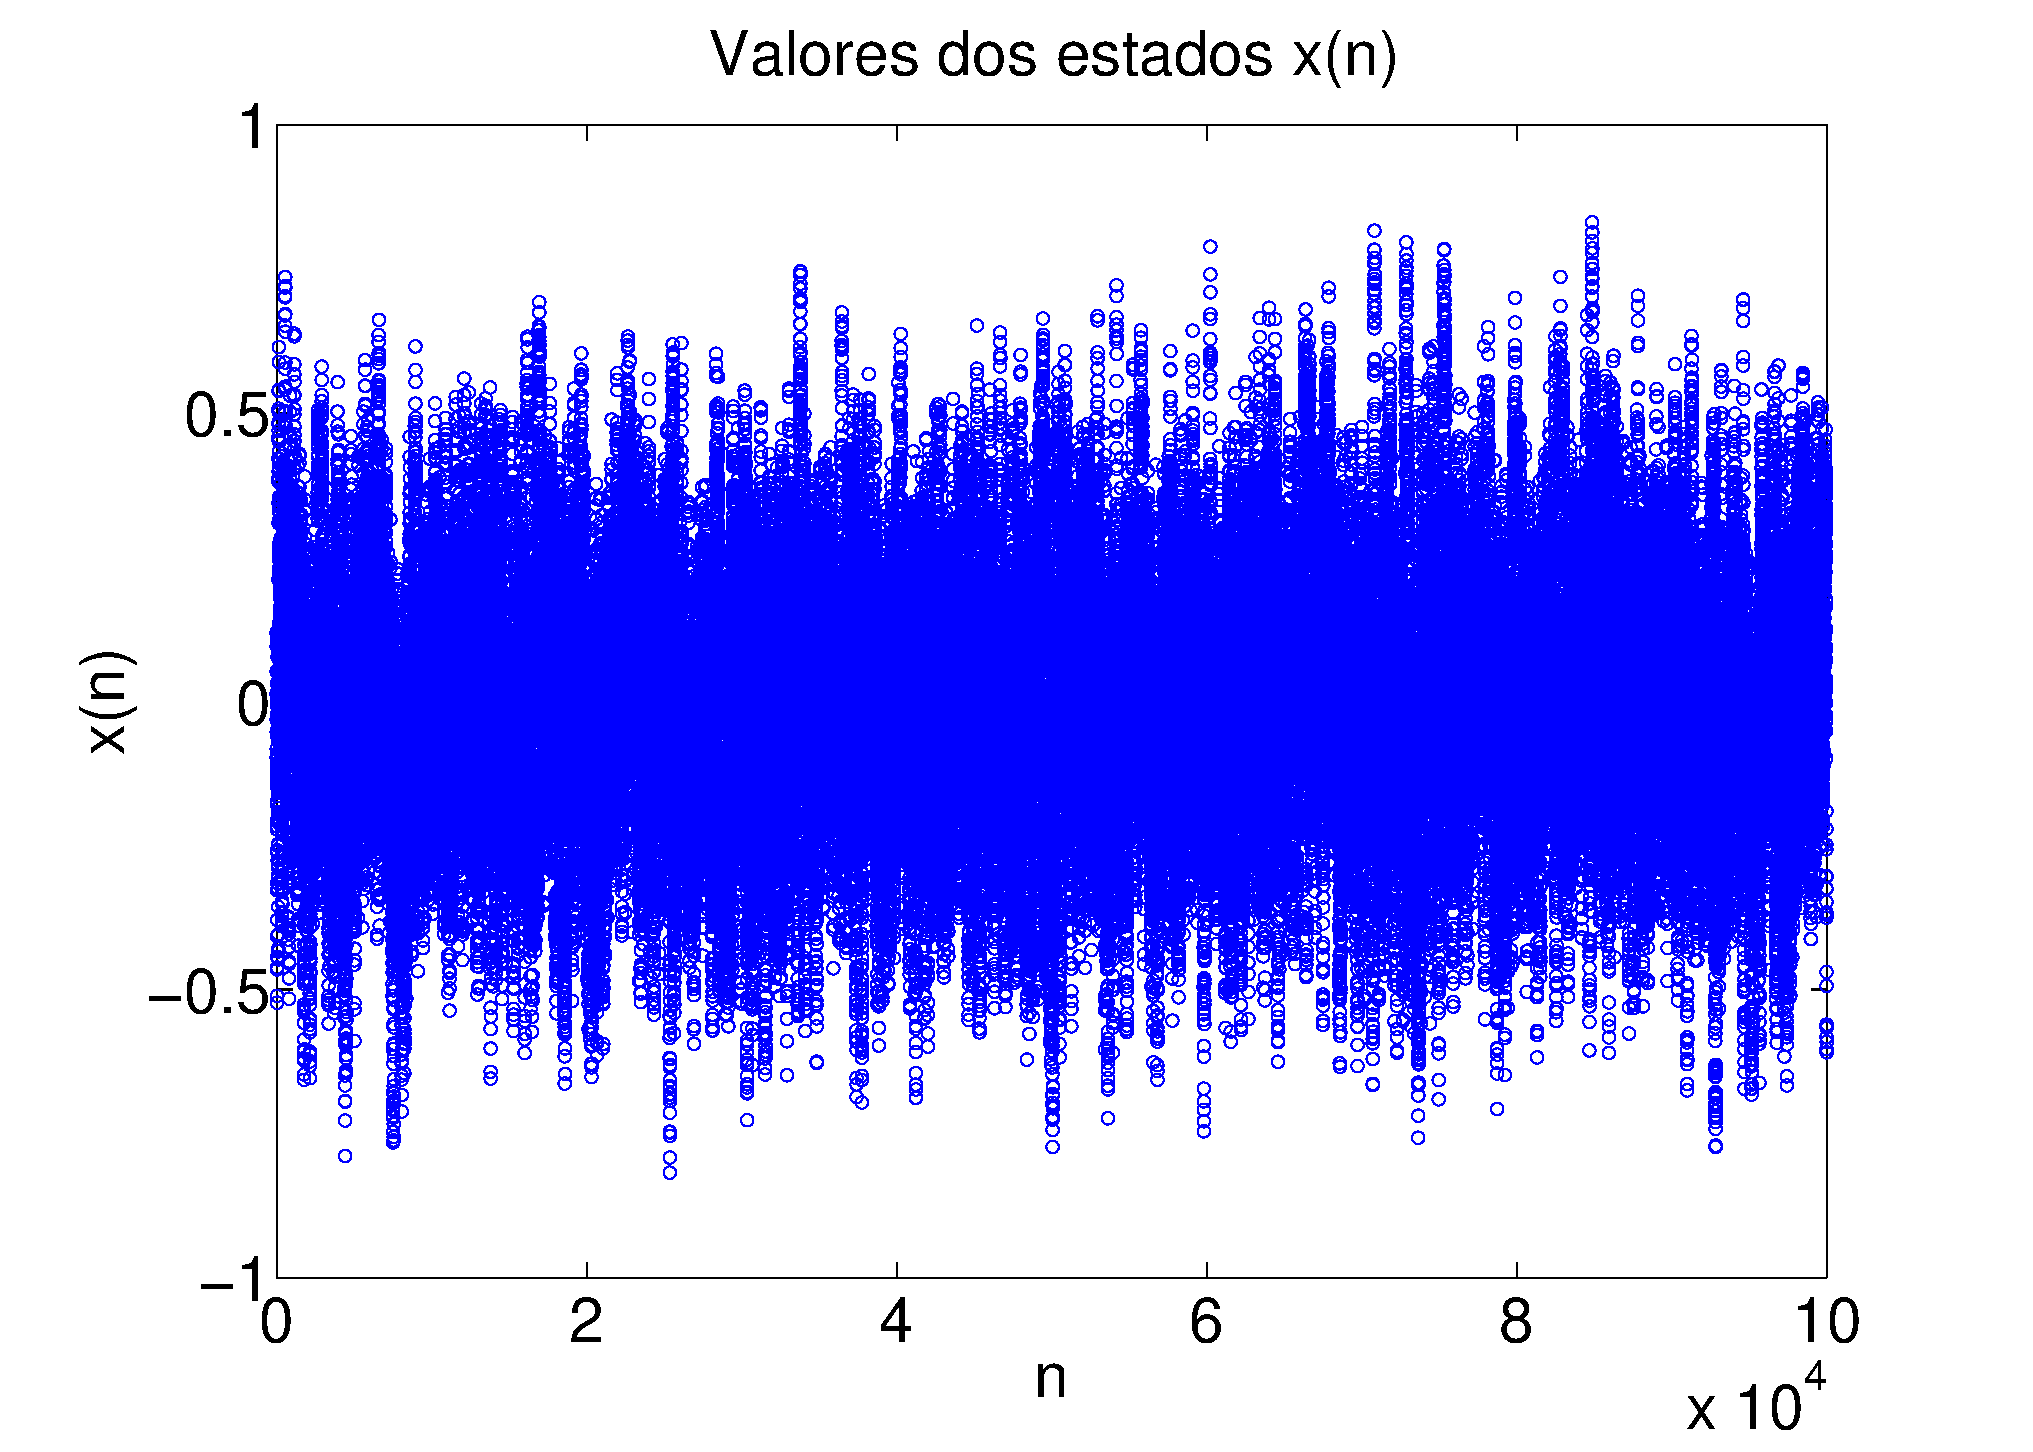
\includegraphics[width = 0.5\textwidth]{Q03_A_valores_x.eps}
		\caption{Amostras $x(n)$ nas 100000 rodadas do algoritmo}
	\end{subfigure}\\[0.5cm]
	\begin{subfigure}{0.4\textwidth}
		\centering
		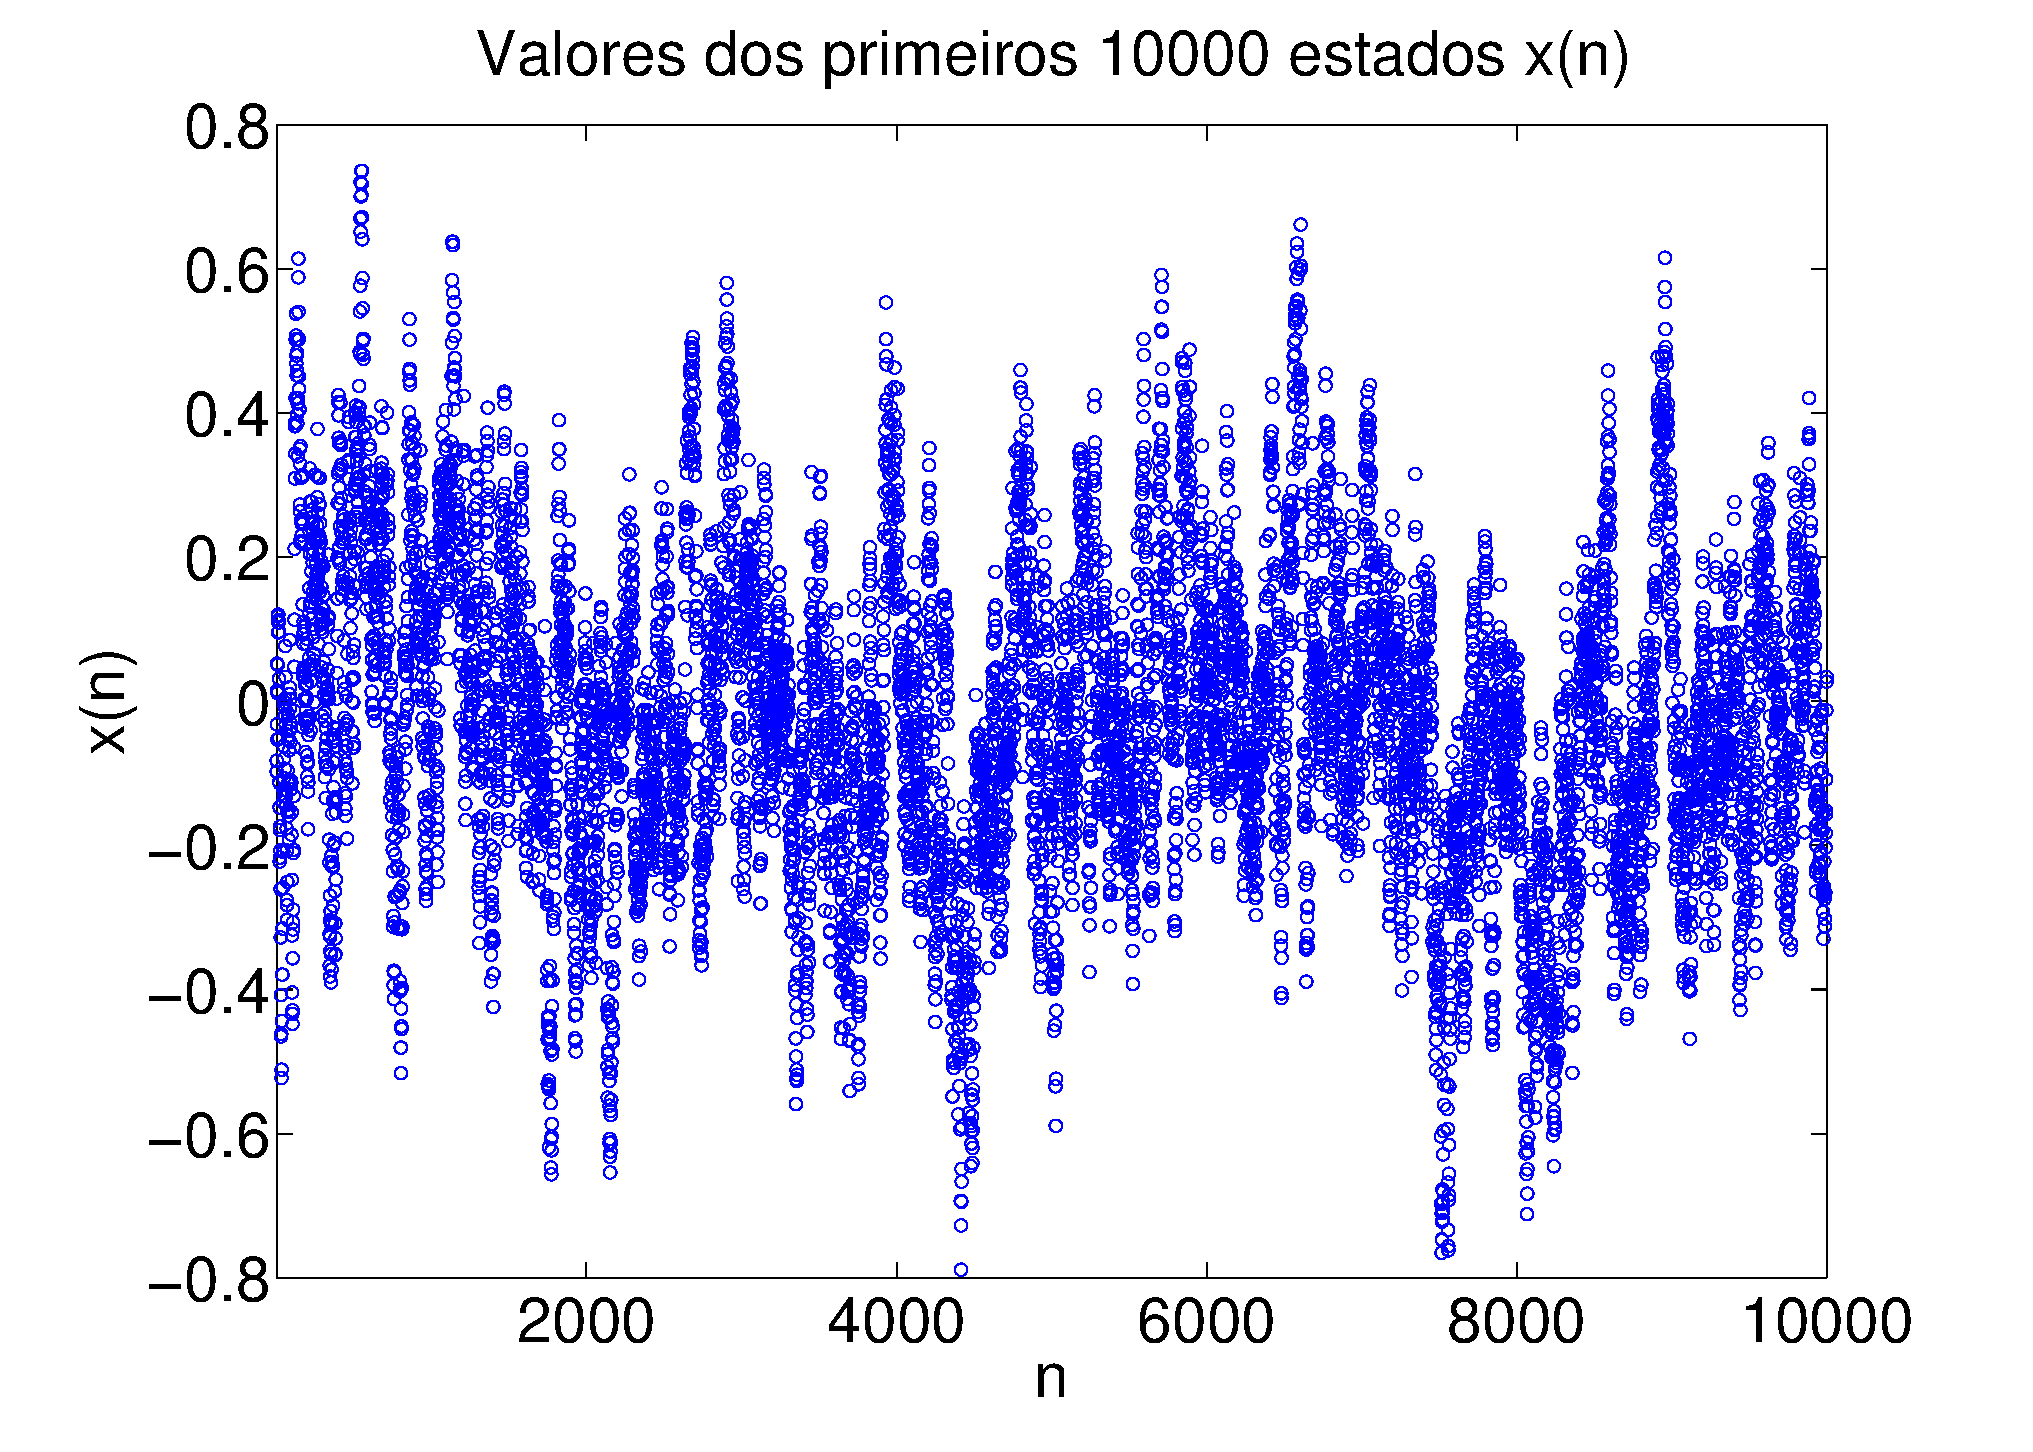
\includegraphics[width = \textwidth]{Q03_A_primeiros_valores_x.eps}
		\caption{Amostras $x(n)$ nas primeiras 10000 rodadas do algoritmo}
	\end{subfigure}
	\hspace{2cm}
	\begin{subfigure}{0.4\textwidth}
		\centering
		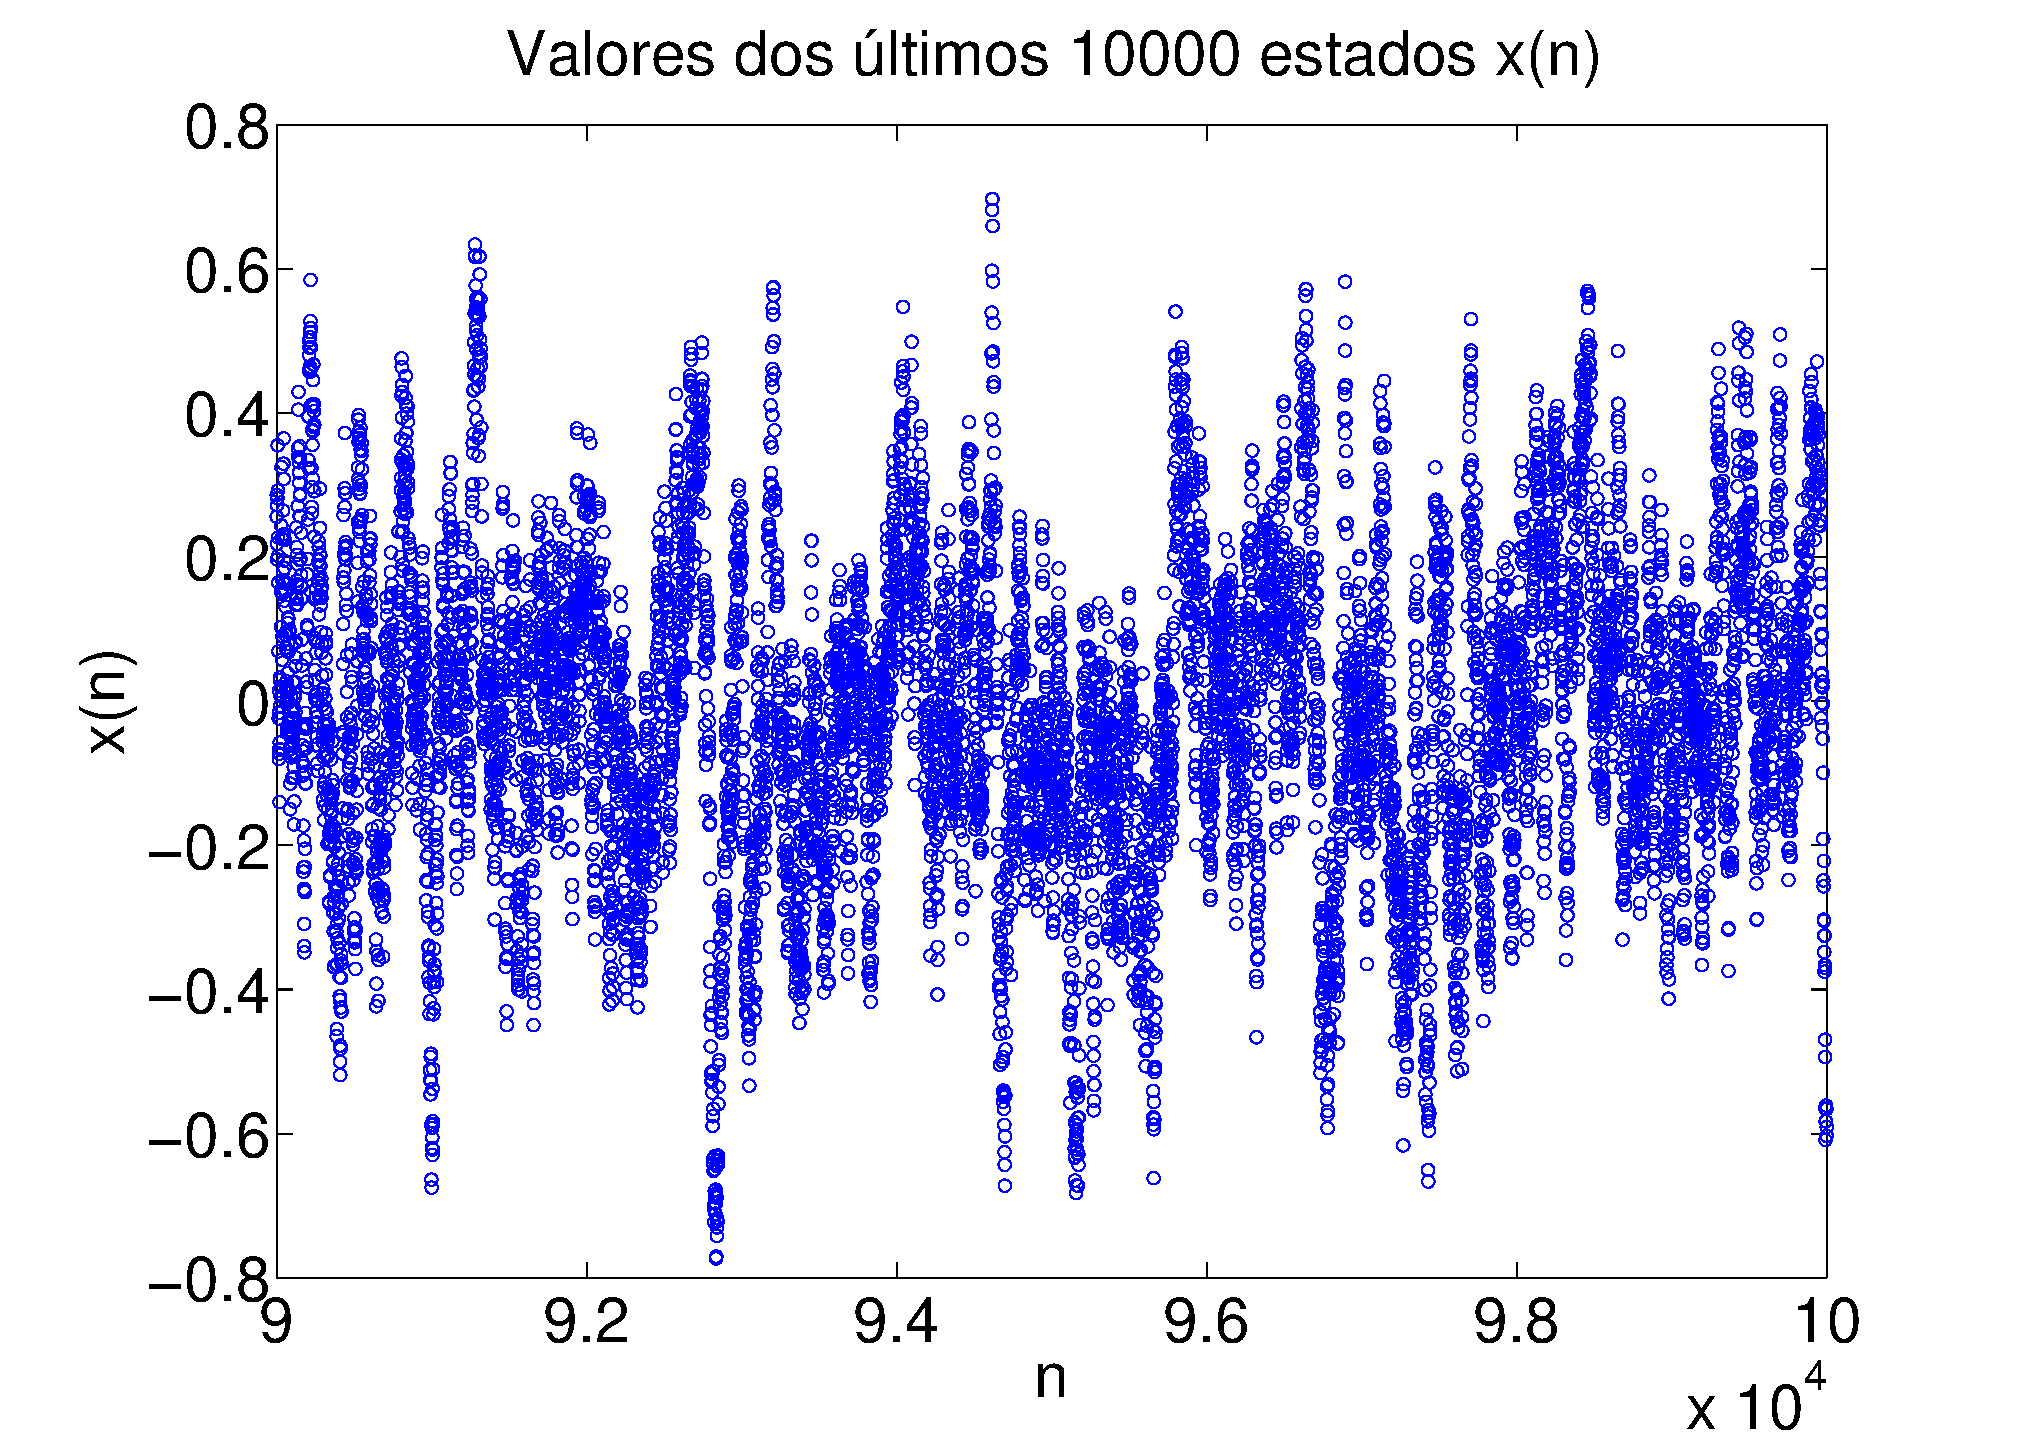
\includegraphics[width = \textwidth]{Q03_A_ultimos_valores_x.eps}
		\caption{Amostras $x(n)$ nas últimas 10000 rodadas do algoritmo}
	\end{subfigure}
	\caption{Valores das amostras $x(n)$}
	\label{fig_estados_x}
\end{figure}

\paragraph{} A Figura \ref{fig_histograma_x} exibe o histograma dos estados $x(n)$ referentes às 10000 últimas iterações do algoritmo. Como era de se esperar, observa-se que esse histograma se assemelha a uma Gaussiana. Calculando a média e a variância dessa distribuição, chega-se aos valores $\mu = -0,014273$, para a média, e $\sigma^2 = 0,050015$, para a variância, os quais são bem próximos aos valores da distribuição Gaussiana em questão ($\mu = 0$ e $\sigma^2 = 0.05$), mostrando que a distribuição dos estados está convergindo para essa Gaussiana. A Figura \ref{fig_histograma_J} exibe a distribuição dos valores da função $J(x) = x^2$, tendo os valores mais prováveis se concentrando no valor mínimo da função (que, no caso, é 0), como era de se esperar.

\begin{figure}[H]
	\centering
	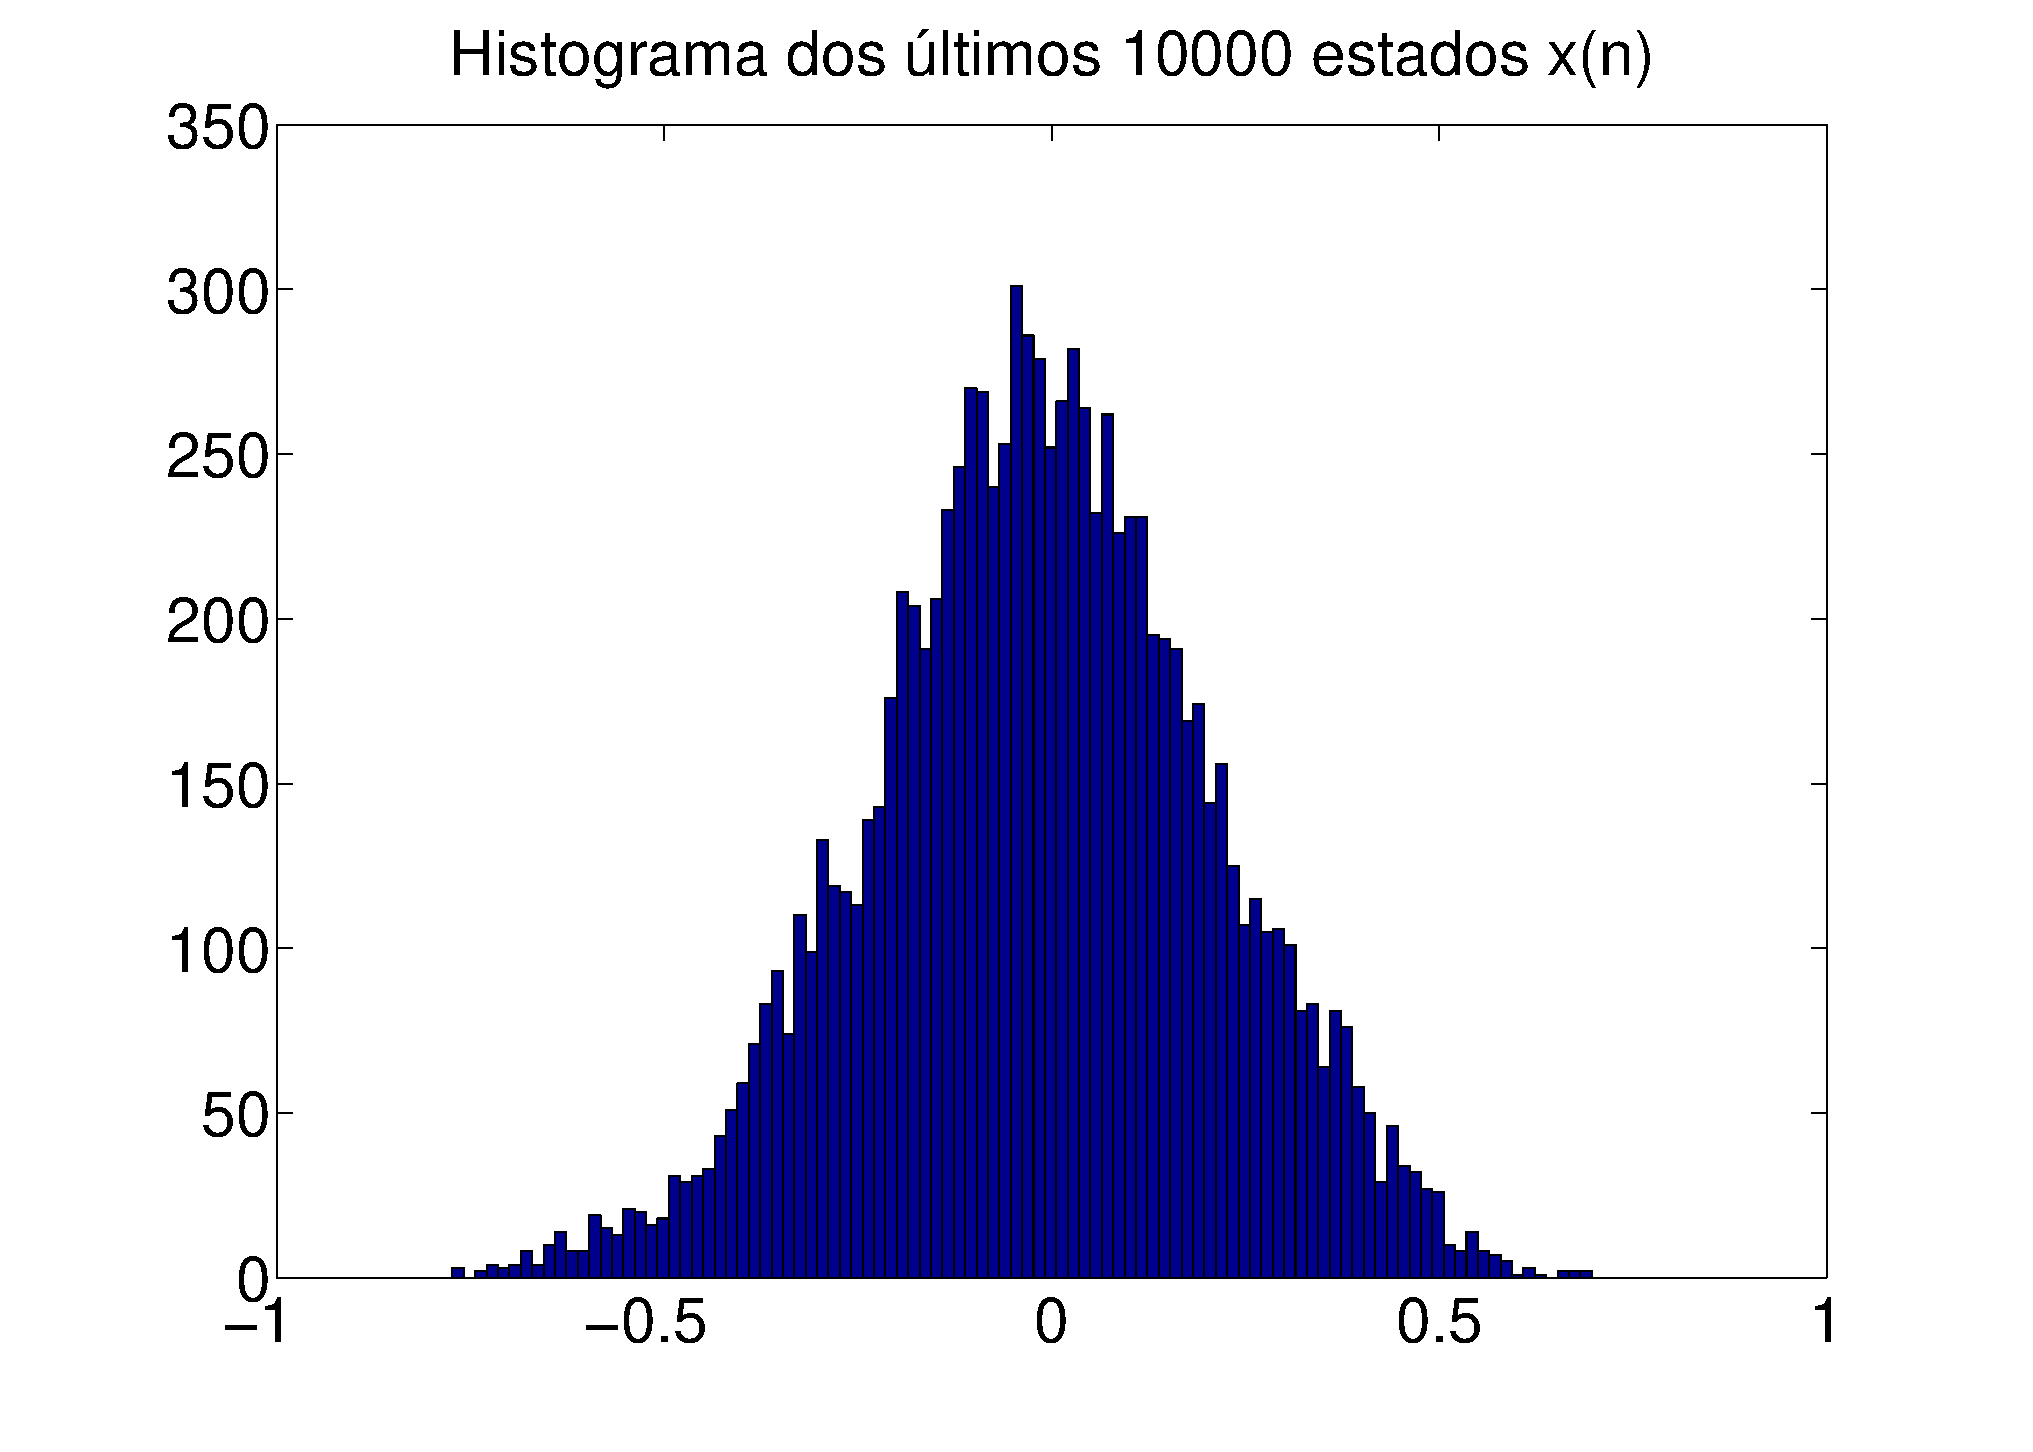
\includegraphics[width = 0.7\textwidth]{Q03_A_histograma_x.eps}
	\caption{Histograma dos últimos 10000 valores dos estados $x(n)$}
	\label{fig_histograma_x}
\end{figure} 

\begin{figure}[H]
	\centering
	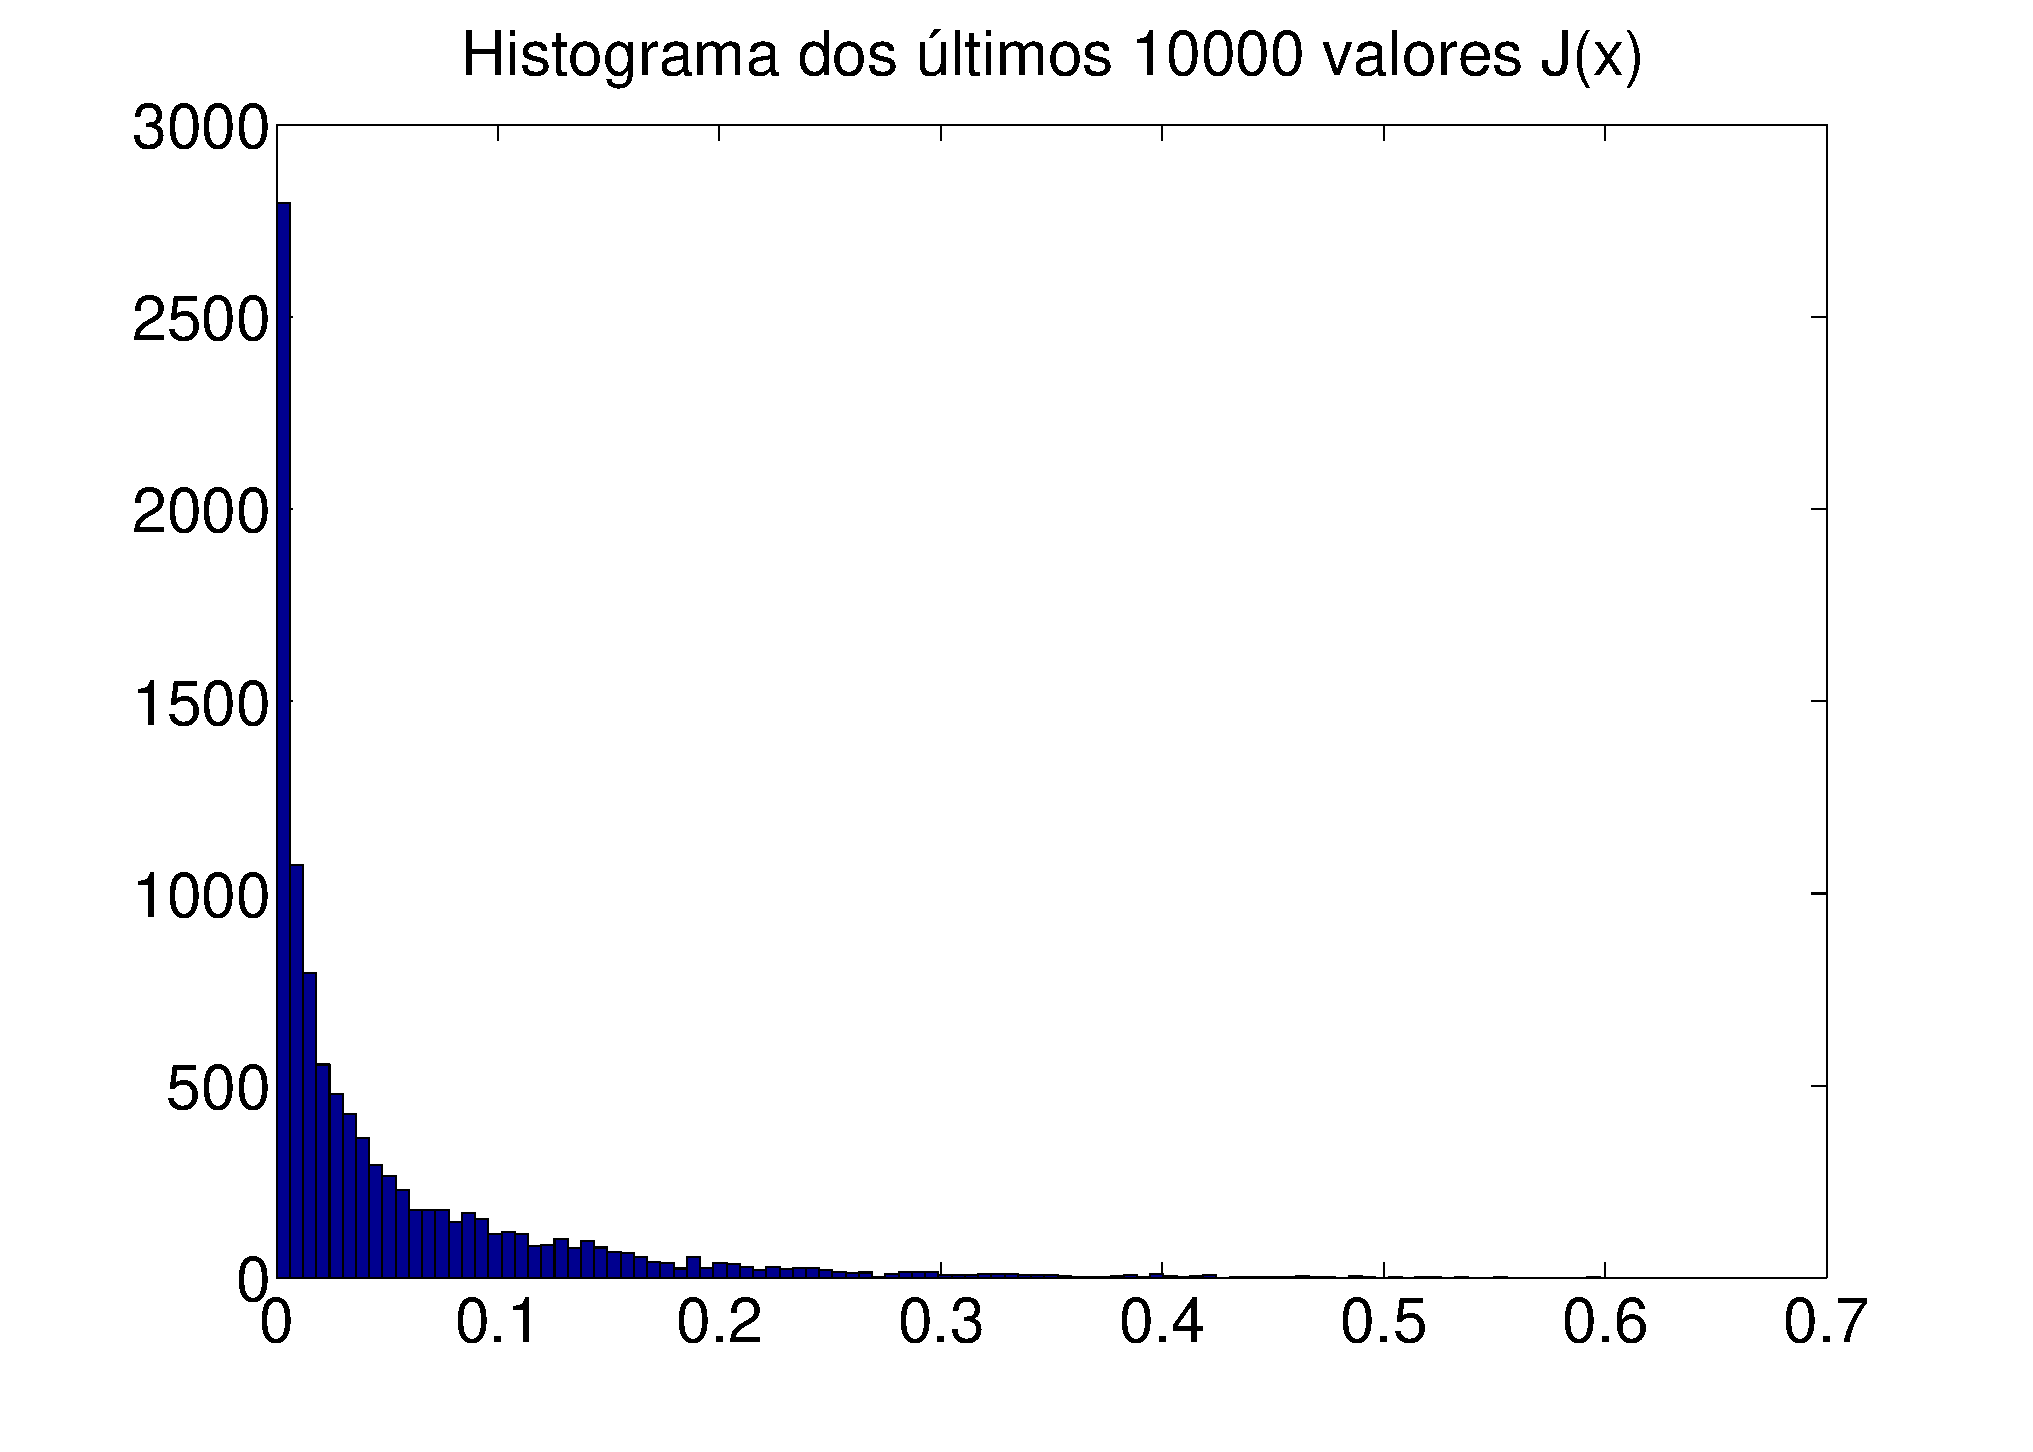
\includegraphics[width = 0.7\textwidth]{Q03_A_histograma_J.eps}
	\caption{Histograma dos últimos 10000 valores da função $J(x)$}
	\label{fig_histograma_J}
\end{figure}

\subsection*{b) Execute manualmente (cálculos no papel) os 10 primeiros passos do algoritmo (ou seja, até n = 10).}

\begin{itemize}

\item Escolhendo aleatoriamente um valor inicial $x(0) = 1$  para a primeira iteração ($n = 1$), temos:

\begin{itemize}

\item[1.] $J_{0} = x(0)^2 = 1^2 = 1$

\item[3.] Escolhe-se aleatoriamente um valor $r$ entre -1 e 1: $r = -0,4$

\item[4.] $\hat{x}(1) = x(0) + 0,1 \times (-0,4) = 1 - 0,04 = 0,96$

\item[5.] $\hat{J}_{1} = \hat{x}(1)^2 = 0,96^2 = 0,9216$

\item[6.] $\Delta J = \hat{J}_{1} - J_{0} = 0,9216 - 1 = -0,0784$

\item[7.] Como $\Delta J < 0$, a transição é aceita diretamente

\item[8.] $J_{1} = \hat{J}_{1} = 0,9216$

\item[9.] $x(1) = \hat{x}(1) = 0,96$

\end{itemize}

\item Começa-se, então, a segunda iteração ($n = 2$):

\begin{itemize}

\item[1.] Escolhe-se aleatoriamente um valor $r$ entre -1 e 1: $r = 0,1$

\item[2.] $\hat{x}(2) = x(1) + 0,1 \times (0,1) = 0,96 + 0,01 = 0,97$

\item[3.] $\hat{J}_{2} = \hat{x}(2)^2 = 0,97^2 = 0,9409$

\item[4.] $\Delta J = \hat{J}_{2} - J_{1} = 0,9409 - 0,9216 = 0,0193$

\item[5.] Como $\Delta J > 0$, escolhe-se aleatoriamente um número $k$ entre 0 e 1, para decidir se a transição será aceita: $k = 0,4$

\item[6.] $e^{\frac{- \Delta J}{T}} = e^{\frac{- 0,0193}{0,1}} = e^{-0,193} \approx 0,8245$

\item[7.] Como $k = 0,4 < 0,8245 = e^{\frac{- \Delta J}{T}}$, a transição é aceita.

\item[8.] $J_{2} = \hat{J}_{2} = 0,9409$

\item[9.] $x(2) = \hat{x}(2) = 0,97$

\end{itemize}

\item Terceira iteração ($n = 3$):

\begin{itemize}

\item[1.] Escolhe-se aleatoriamente um valor $r$ entre -1 e 1: $r = 0,5$

\item[2.] $\hat{x}(3) = x(2) + 0,1 \times (0,5) = 0,97 + 0,05 = 1,02$

\item[3.] $\hat{J}_{3} = \hat{x}(3)^2 = 1,02^2 = 1,0404$

\item[4.] $\Delta J = \hat{J}_{3} - J_{2} = 1,0404 - 0,9409 = 0,0995$

\item[5.] Como $\Delta J > 0$, escolhe-se aleatoriamente um número $k$ entre 0 e 1, para decidir se a transição será aceita: $k = 0,1$

\item[6.] $e^{\frac{- \Delta J}{T}} = e^{\frac{- 0,0995}{0,1}} = e^{-0,995} \approx 0,37$

\item[7.] Como $k = 0,1 < 0,37 = e^{\frac{- \Delta J}{T}}$, a transição é aceita.

\item[8.] $J_{3} = \hat{J}_{3} = 1,0404$

\item[9.] $x(3) = \hat{x}(3) = 1,02$

\end{itemize}

\item Quarta iteração ($n = 4$):

\begin{itemize}

\item[1.] Escolhe-se aleatoriamente um valor $r$ entre -1 e 1: $r = 0,3$

\item[2.] $\hat{x}(4) = x(3) + 0,1 \times (0,3) = 1,02 + 0,03 = 1,05$

\item[3.] $\hat{J}_{4} = \hat{x}(4)^2 = 1,05^2 = 1,1025$

\item[4.] $\Delta J = \hat{J}_{4} - J_{3} = 1,1025 - 1,0404 = 0,0621$

\item[5.] Como $\Delta J > 0$, escolhe-se aleatoriamente um número $k$ entre 0 e 1, para decidir se a transição será aceita: $k = 0,6$

\item[6.] $e^{\frac{- \Delta J}{T}} = e^{\frac{- 0,0621}{0,1}} = e^{-0,621} \approx 0,54$

\item[7.] Como $k = 0,6 > 0,54 = e^{\frac{- \Delta J}{T}}$, a transição não é aceita.

\item[8.] $J_{4} = J_{3} = 1,0404$

\item[9.] $x(4) = x(3) = 1,02$

\end{itemize}

\item Quinta iteração ($n = 5$):

\begin{itemize}

\item[1.] Escolhe-se aleatoriamente um valor $r$ entre -1 e 1: $r = -0,8$

\item[2.] $\hat{x}(5) = x(4) + 0,1 \times (-0,8) = 1,02 - 0,08 = 0,94$

\item[3.] $\hat{J}_{5} = \hat{x}(5)^2 = 0,94^2 = 0,8836$

\item[4.] $\Delta J = \hat{J}_{5} - J_{4} = 0,8836 - 1,0404 = -0,1568$

\item[5.] Como $\Delta J < 0$, a transição é aceita.

\item[6.] $J_{5} = \hat{J}_{5} = 0,8836$

\item[7.] $x(5) = \hat{x}(5) = 0,94$

\end{itemize}

\item Sexta iteração ($n = 6$)

\begin{itemize}

\item[1.] Escolhe-se aleatoriamente um valor $r$ entre -1 e 1: $r = 0,7$

\item[2.] $\hat{x}(6) = x(5) + 0,1 \times (0,7) = 0,94 + 0,07 = 1,01$

\item[3.] $\hat{J}_{6} = \hat{x}(6)^2 = 1,01^2 = 1,0201$

\item[4.] $\Delta J = \hat{J}_{6} - J_{5} = 1,0201 - 0,8836 = 0,1365$

\item[5.] Como $\Delta J > 0$, escolhe-se aleatoriamente um número $k$ entre 0 e 1, para decidir se a transição será aceita: $k = 0,3$

\item[6.] $e^{\frac{- \Delta J}{T}} = e^{\frac{- 0,1365}{0,1}} = e^{-1,365} \approx 0,26$

\item[7.] Como $k = 0,3 > 0,26 = e^{\frac{- \Delta J}{T}}$, a transição não é aceita.

\item[8.] $J_{6} = J_{5} = 0,8836$

\item[9.] $x(6) = x(5) = 0,94$

\end{itemize}

\item Sétima iteração ($n = 7$)

\begin{itemize}

\item[1.] Escolhe-se aleatoriamente um valor $r$ entre -1 e 1: $r = -0,1$

\item[2.] $\hat{x}(7) = x(6) + 0,1 \times (-0,1) = 0,94 - 0,01 = 0,93$

\item[3.] $\hat{J}_{7} = \hat{x}(7)^2 = 0,93^2 = 0,8649$

\item[4.] $\Delta J = \hat{J}_{7} - J_{6} = 0,8649 - 0,8836 = -0,0187$

\item[5.] Como $\Delta J < 0$, a transição é aceita

\item[6.] $J_{7} = \hat{J}_{7} = 0,8649$

\item[7.] $x(7) = \hat{x}(7) = 0,93$

\end{itemize}

\item Oitava iteração ($n = 8$)

\begin{itemize}

\item[1.] Escolhe-se aleatoriamente um valor $r$ entre -1 e 1: $r = -0,8$

\item[2.] $\hat{x}(8) = x(7) + 0,1 \times (-0,8) = 0,93 - 0,08 = 0,85$

\item[3.] $\hat{J}_{8} = \hat{x}(8)^2 = 0,85^2 = 0,7225$

\item[4.] $\Delta J = \hat{J}_{8} - J_{7} = 0,7225 - 0,8649 = -0,1424$

\item[5.] Como $\Delta J < 0$, a transição é aceita

\item[6.] $J_{8} = \hat{J}_{8} = 0,7225$

\item[7.] $x(8) = \hat{x}(8) = 0,85$

\end{itemize}

\item Nona iteração ($n = 9$)

\begin{itemize}

\item[1.] Escolhe-se aleatoriamente um valor $r$ entre -1 e 1: $r = 0,8$

\item[2.] $\hat{x}(9) = x(8) + 0,1 \times (0,8) = 0,93 + 0,08 = 1,01$

\item[3.] $\hat{J}_{9} = \hat{x}(9)^2 = 1,01^2 = 1,0201$

\item[4.] $\Delta J = \hat{J}_{9} - J_{8} = 1,0201 - 0,7225 = 0,2976$

\item[5.] Como $\Delta J > 0$, escolhe-se aleatoriamente um número $k$ entre 0 e 1, para decidir se a transição será aceita: $k = 0,5$

\item[6.] $e^{\frac{- \Delta J}{T}} = e^{\frac{- 0,2976}{0,1}} = e^{-2,976} \approx 0,05$

\item[7.] Como $k = 0,5 > 0,05 = e^{\frac{- \Delta J}{T}}$, a transição não é aceita.

\item[8.] $J_{9} = J_{8} = 0,7225$

\item[9.] $x(9) = x(8) = 0,85$

\end{itemize}

\item Décima iteração ($n = 10$)

\begin{itemize}

\item[1.] Escolhe-se aleatoriamente um valor $r$ entre -1 e 1: $r = -0,6$

\item[2.] $\hat{x}(10) = x(9) + 0,1 \times (-0,6) = 0,85 - 0,06 = 0,79$

\item[3.] $\hat{J}_{10} = \hat{x}(10)^2 = 0,79^2 = 0,6241$

\item[4.] $\Delta J = \hat{J}_{10} - J_{9} = 0,6241 - 0,7225 = -0,0984$

\item[5.] Como $\Delta J < 0$, a transição é aceita

\item[8.] $J_{10} = \hat{J}_{10} = 0,6241$

\item[9.] $x(10) = \hat{x}(10) = 0,79$

\end{itemize}

\end{itemize}

\section*{4. Escrever um programa S.A. (pode ser pseudo-código) para minimizar a função escalar $J(x) = -x + 100(x - 0.2)^2(x - 0.8)^2$. Começando de $x(0) = 0$ e utilizando geradores de números aleatórios (um uniforme e outro Gaussiano), calcule manualmente os 10 primeiros valores de $x(n)$ gerados pelo S.A.}

\paragraph{} O pseudo-código do S.A, que implementa a solução dessa questão, encontra-se descrito a seguir:

\begin{lstlisting}
$x_i \leftarrow 0$
$J_i \leftarrow -x_i + 100(x_i - 0,2)^2(x_i - 0.8)^2$
$T0 \leftarrow 1$
$k_{max} \leftarrow 9$ (quantidade de temperaturas que serao utilizadas)
$N \leftarrow 100000$ (numero de iteracoes no Algoritmo de Metropolis)

para $k = 0$ ... $k_{max}$
	$T = T0(0,9)^k$
	para $i = 1$ ... $N$
		$r \leftarrow $ amostra de uma variavel aleatoria simetrica (no caso, uniforme ou Gaussiana)
		$\hat{x}_{i+1} \leftarrow x_i + \epsilon \times r$
		$\hat{J}_{i+1} = -\hat{x}_{i+1} + 100(\hat{x}_{i+1} - 0,2)^2(\hat{x}_{i+1} - 0.8)^2$
		$\Delta J = \hat{J}_{i+1} - J_i$
		Se $\Delta J < 0$
			x_{i+1} = \hat{x}_{i+1}
			J_{i+1} = \hat{J}_{i+1}
		Senao
			$\beta \leftarrow$ amostra de uma variavel aleatoria uniforme entre [0,1]
			Se $\beta < e^{\frac{- \Delta J}{T}}$
				x_{i+1} = \hat{x}_{i+1}
				J_{i+1} = \hat{J}_{i+1}
			Senao
				x_{i+1} = x_i
				J_{i+1} = J_i
			Fim Se
		Fim Se
	Fim Loop
	
	$x_{finais}(k) = x_i$ (guarda os valores x_i da ultima iteracao do Algoritmo de Metropolis)
	$k \leftarrow k + 1$
Fim Loop
		
\end{lstlisting}

\paragraph{} O código, em MATLAB, que minimiza a função $J(x)$ é mostrado a seguir:

\begin{verbatim}
x_atual = 0;
epsilon = 0.1;

T0 = 1;
N = 100000;
x = zeros(1,N);
J = zeros(1,N);
J_min = inf;
X_min = inf;

X = [];
J_rodadas = [];
k = 0;
interrompe = 0;
indice_T = 1;

while (~interrompe)
    
    T_atual = (0.9^k) * T0;
    
    disp(['T: ' num2str(T_atual)])
    
%     if T_atual < 0.1
%         interrompe = 1;
%     end

    if k > 9
        interrompe = 1;
    end
    
    T(indice_T) = T_atual;
    indice_T = indice_T + 1;
    
    if (~interrompe)
    
        for i = 1:N

            x(i) = x_atual;
            J_atual = - x_atual + 100 * ((x_atual - 0.2).^2) .* ((x_atual - 0.8).^2);
            J(i) = J_atual;

            if J_atual < J_min
                J_min = J_atual;
                X_min = x_atual;
            end

            r = random('unif', -1, 1);
%             r = random('norm', 0, 1);
            x_futuro = x_atual + epsilon * r;
            J_futuro = - x_futuro + 100 * ((x_futuro - 0.2).^2) .* ((x_futuro - 0.8).^2);
            J_dif = J_futuro - J_atual;

            if J_dif < 0
                x_atual = x_futuro;
            else
                beta = rand(1,1);

                if beta < exp(-(J_dif)/T_atual)
                    x_atual = x_futuro;
                end
            end        
        end

        X = [X; x];
        J_rodadas = [J_rodadas; J];

        k = k + 1;
    end
    
end


\end{verbatim}

\paragraph{} Os dez primeiros valores de $x(n)$ podem ser obtidos trocando a condição de parada do loop da temperatura. Em vez de utilizar um valor de temperatura, utiliza-se o valor de k para essa condição. No caso, como $k = 0$ inicialmente, o loop deve parar quando $k > 9$. Os primeiros 10 valores de $x(n)$ estão exibidos a seguir, para cada uma das diferentes variáveis aleatórias utilizadas (uniforme e Gaussiana). Os 10 primeiros valores do algoritmo correspondem aos últimos estados $x(n)$ de cada uma das 10 temperaturas utilizadas.

\begin{verbatim}
% Resultados dos 10 primeiros x(n) usando variável aleatoria uniforme
% 
%  X(:,end)
% 
% ans =
% 
%     0.3041
%     0.1229
%     0.1448
%     0.8402
%     0.1417
%     0.6628
%     0.8097
%     0.7775
%     0.2803
%     0.7753

% Resultados dos 10 primeiros x(n) usando variável aleatoria Gaussiana
% 
% X(:,end)
% 
% ans =
% 
%     0.9989
%     0.6901
%     0.7380
%     0.6671
%     0.7535
%     0.7659
%     0.8294
%     0.8342
%     0.4339
%     0.8992
\end{verbatim}

\section*{5. Proponha uma função de até 4 variáveis cujo ponto mínimo você conheça, e encontre este ponto mínimo utilizando S.A (neste exercício, basta entregar o código escrito).}

\paragraph{} A função escolhida foi: $J(x) = [(x+2)^2 - 3][10(x-3)^2 + 5]$. Seu ponto mínimo global ocorre em $x_{min} \approx -2,49$ e vale $J(x_{min}) \approx -845,64$. O código e seu resultado são exibidos a seguir:

\begin{verbatim}
x_atual = 0;
epsilon = 0.1;

T0 = 1;
N = 100000;
x = zeros(1,N);
J = zeros(1,N);
J_min = inf;
X_min = inf;

X = [];
J_rodadas = [];
k = 0;
interrompe = 0;
indice_T = 1;

while (~interrompe)
    
    T_atual = (0.9^k) * T0;
    
    disp(['T: ' num2str(T_atual)])
    
    if T_atual < 0.1
        interrompe = 1;
    end
    
    T(indice_T) = T_atual;
    indice_T = indice_T + 1;
    
    if (~interrompe)
    
        for i = 1:N

            x(i) = x_atual;
            J_atual = (((x_atual + 2) ^ 2) - 3) * (10 * ((x_atual - 3) ^ 2) + 5);
            J(i) = J_atual;

            if J_atual < J_min
                J_min = J_atual;
                X_min = x_atual;
            end

            r = random('unif', -1, 1);
            x_futuro = x_atual + epsilon * r;
            J_futuro = (((x_futuro + 2) ^ 2) - 3) * (10 * ((x_futuro - 3) ^ 2) + 5);
            J_dif = J_futuro - J_atual;

            if J_dif < 0
                x_atual = x_futuro;
            else
                beta = rand(1,1);

                if beta < exp(-(J_dif)/T_atual)
                    x_atual = x_futuro;
                end
            end        
        end

        X = [X; x];
        J_rodadas = [J_rodadas; J];

        k = k + 1;
    end
    
end

% Resultados do código
% 
% J_min = -845.6411
% X_min = -2.4936
\end{verbatim}

\paragraph{} A Figura \ref{fig_histograma_J_q_5} mostra a distribuição das energias nas 10000 últimas iterações do algoritmo na última temperatura executada ($T = 0.1094$). Como se observa, os valores que mais ocorreram foram aqueles próximos ao ponto de mínimo global da função.

\begin{figure}[H]
	\centering
	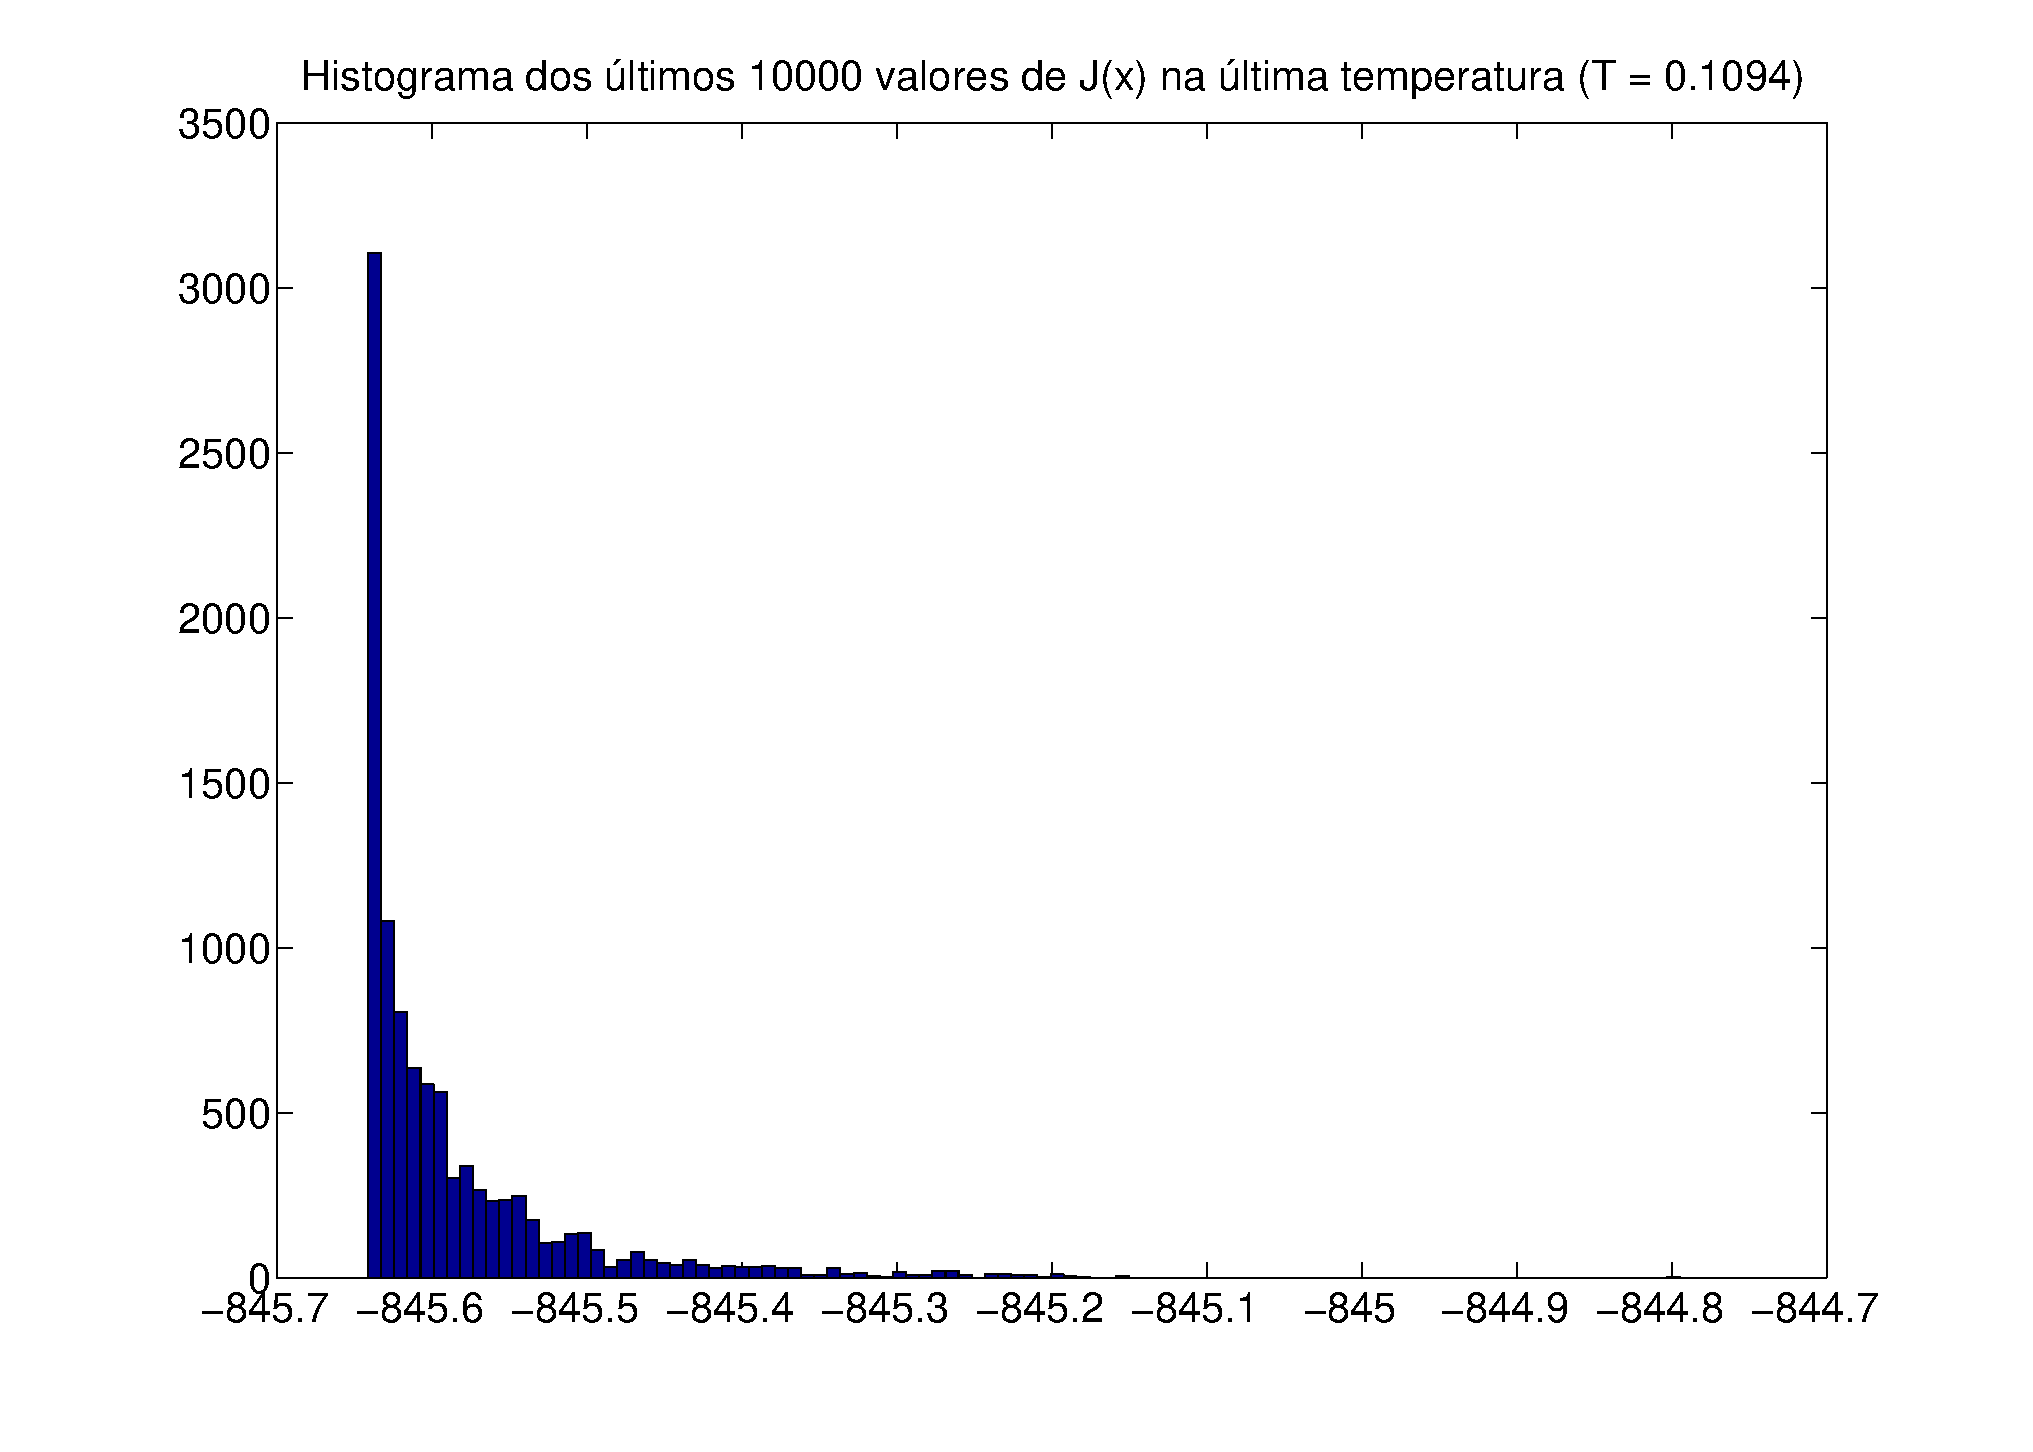
\includegraphics[width = 0.7\textwidth]{Q05_histograma_J.eps}
	\caption{Distribuição dos valores da função $J(x)$ nas últimas 10000 iterações da última temperatura $T \approx 0,1094$}
	\label{fig_histograma_J_q_5}
\end{figure}

\paragraph{} A Figura \ref{fig_histograma_x_q_5} mostra a distribuição de estados $x(n)$, também obtidos nas 10000 últimas iterações do algoritmo na última temperatura. Como era de se esperar, os valores mais observados se concentraram em torno da coordenada que resulta no ponto de mínimo da função. O pico desse histograma, inclusive, encontra-se em $x = -2,49$, que, de fato, é a coordenada do mínimo da função $J(x)$.

\begin{figure}
	\centering
	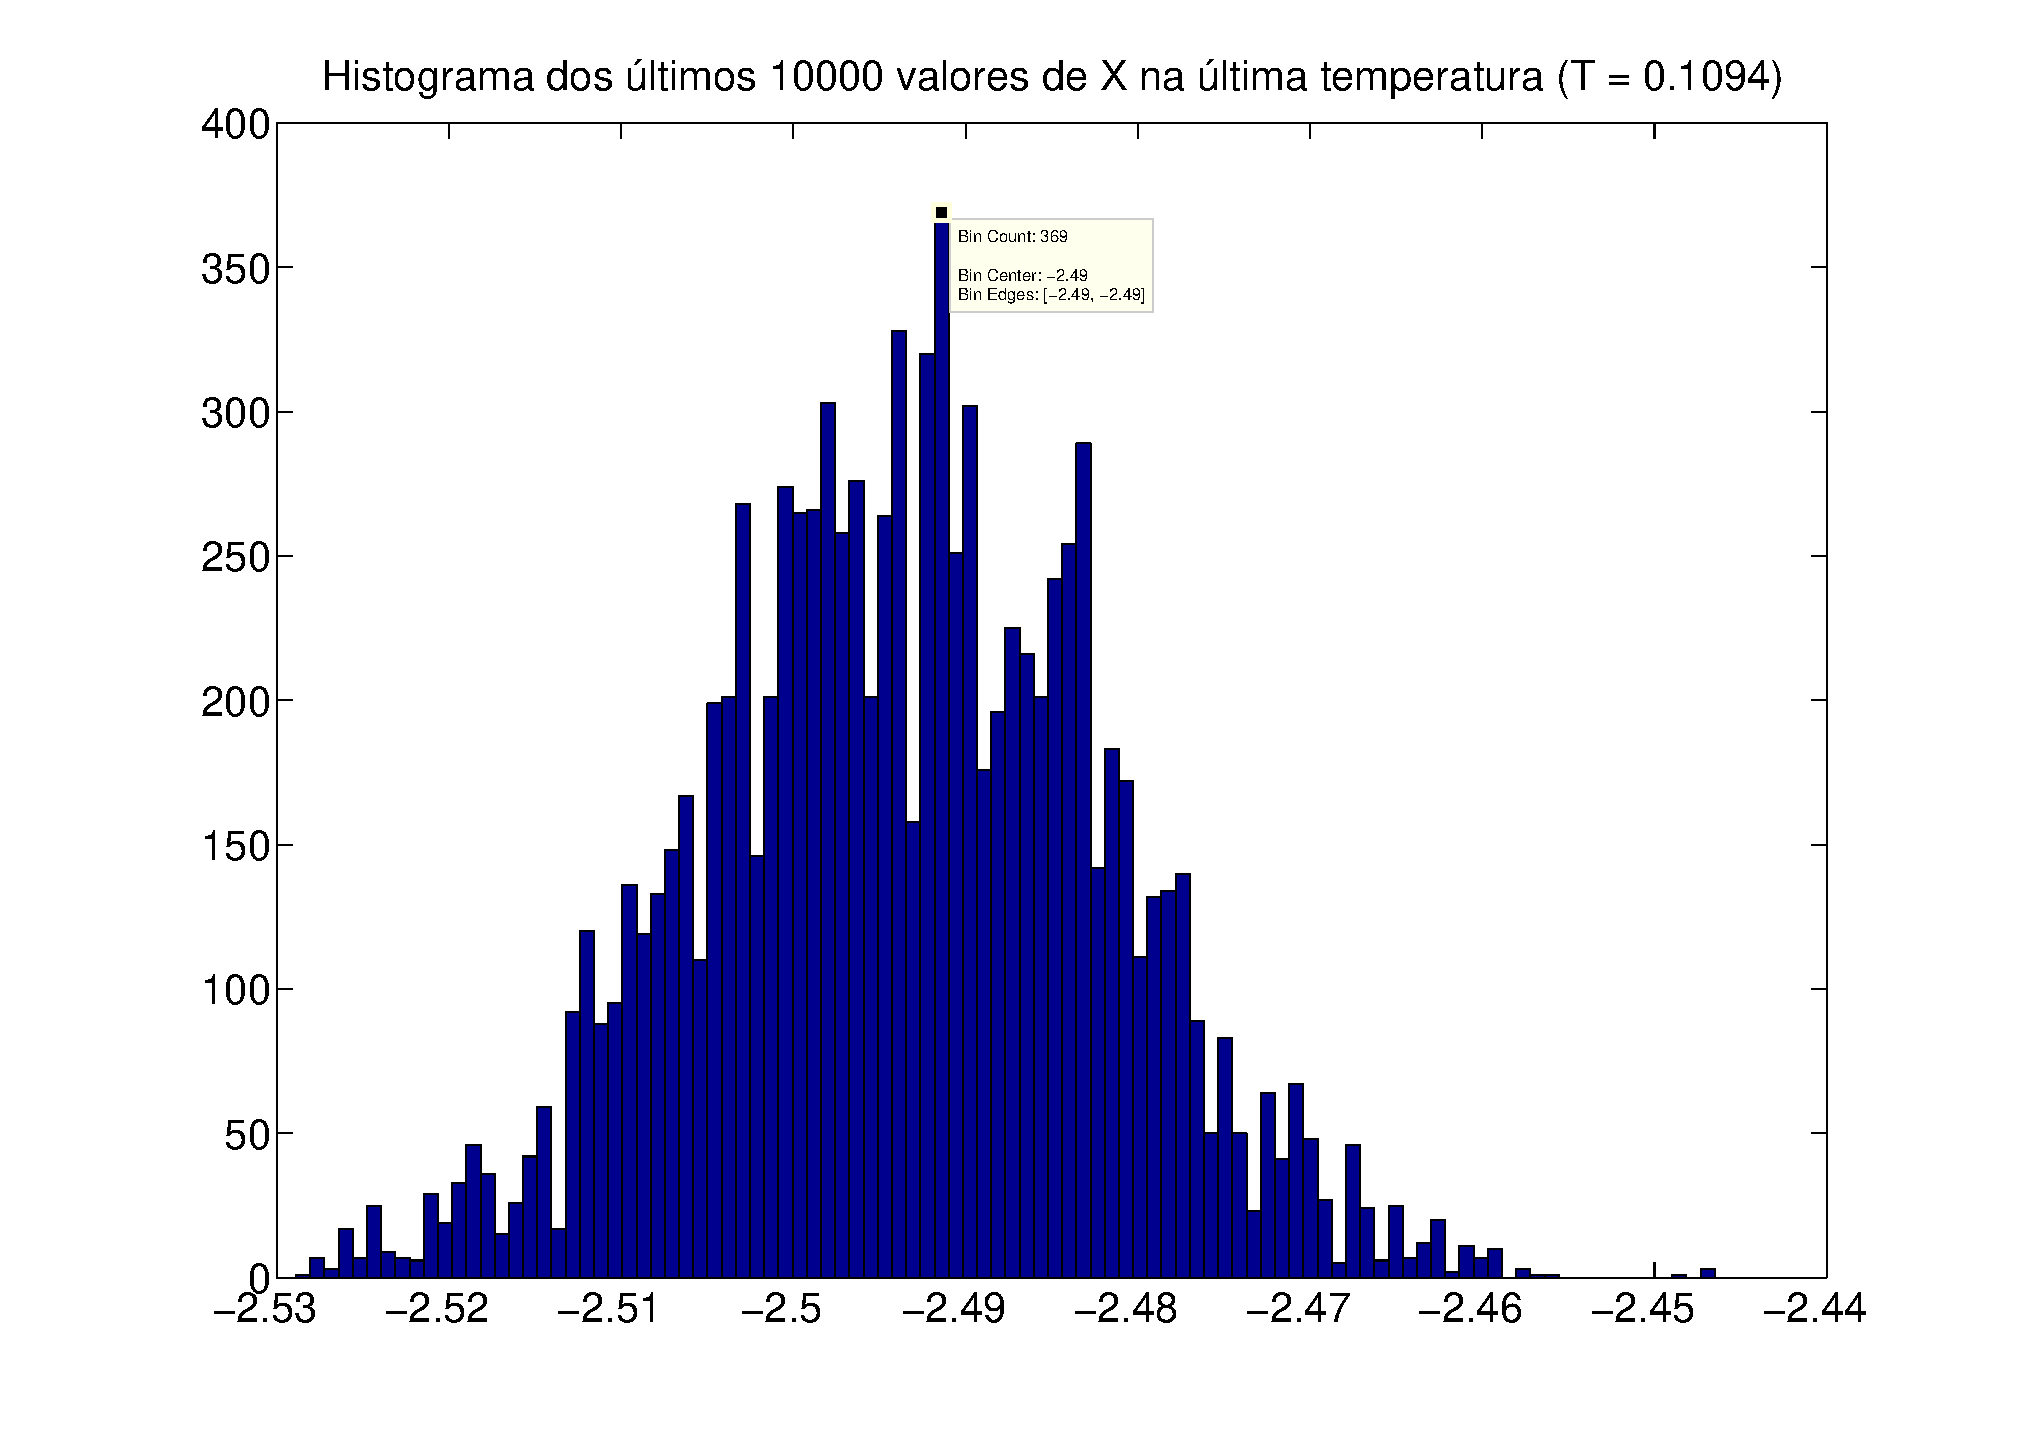
\includegraphics[width = 0.7\textwidth]{Q05_histograma_x.eps}
	\caption{Distribuição dos estados $x(n)$ nas últimas 10000 iterações da última temperatura ($T \approx 0,1094$)}
	\label{fig_histograma_x_q_5}
\end{figure}

\end{document}